%% Scientific Reports (Nature Portfolio) version.
%% Source of every number: paper/submission/main.tex (IEEE-style version).
%% Blanks only the authors can fill are marked [TO BE FILLED ...].
\documentclass[pdflatex,sn-nature]{sn-jnl}

\usepackage{graphicx}
\usepackage{amsmath,amssymb}
\usepackage{booktabs}
\usepackage{textcomp}
\usepackage{xcolor}

\raggedbottom
\hypersetup{hidelinks}
\emergencystretch=3em
\vbadness=10000 % hides the harmless underfull page-footer box of sn-jnl.cls (it fires on every page)
\unnumbered

\newcommand{\dnet}{\mathbf{d}_{\mathrm{net}}}
\newcommand{\dgeo}{\mathbf{d}_{\mathrm{geo}}}
\newcommand{\tbf}[1]{\textbf{#1}}

\begin{document}

\title[Observability-gated visual--inertial odometry]{Observability-gated fusion of sensor measurements and a neural network improves learned visual--inertial odometry}

\author*[1]{\fnm{Nada} \sur{El Madah}}\email{nadaelmadah@mans.edu.eg}
\author[1]{\fnm{Magdy} \sur{Zakaria}}
\author[1]{\fnm{Samir} \sur{Elmougy}}
\author[1]{\fnm{Shahenda} \sur{Sarhan}}
\author[1]{\fnm{Mohamed} \sur{Handosa}}
\author[1]{\fnm{Rasha Elsayed} \sur{Sakr}}

\affil[1]{\orgdiv{Computer Science}, \orgname{Mansoura University}, \orgaddress{\city{Mansoura}, \country{Egypt}}}

\abstract{Where satellite positioning is unavailable, robots, drones and headsets can track their motion with a camera and an inertial sensor (visual--inertial odometry). Recent systems train one neural network to predict the whole motion, although the sensors already measure much of it. Replacing one predicted component at a time by ground truth showed which fails: rotation and step length on a driving dataset (KITTI), direction of travel on a drone dataset (EuRoC). It also revealed a 4\% timing error in inertial files distributed with several released models (image interval about 104 ms, not 100 ms). We then built an observability gate that, for each pair of frames and component, uses the sensor measurement where observable and the frozen network elsewhere. On KITTI it lowers the translation error of a published model from 1.96\% to 1.56\%, and of released models from three further families by 45--51\%. On EuRoC and TUM-VI it reduces learned networks' error, yet a classical system (ORB-SLAM3) is about 22 times more accurate on EuRoC, so this is a diagnosis, not a state of the art. A post-hoc revision fixed a TUM-VI failure but was no better on an unseen sequence. We report every failure.}

\maketitle

\section{Introduction}\label{sec:intro}

Satellite positioning does not work inside buildings, mines or tunnels, so a robot, a drone or an augmented-reality headset that moves there must estimate its own motion from on-board sensors. A common choice is a camera combined with an inertial measurement unit (IMU), a small sensor, present in every smartphone, whose gyroscope measures rotation and whose accelerometer measures acceleration. Tracking motion with these two sensors is called visual--inertial odometry (VIO). For each pair of consecutive camera frames it estimates how the camera rotated, in which direction it moved and how far it moved (the step length).

Classical VIO integrates the gyroscope between frames, using accurate timestamps and a calibrated offset between camera and IMU, inside filters\cite{Mourikis2007} or optimisation-based systems\cite{Leutenegger2015,Qin2018,Campos2021,Furgale2013,Qin2018b}. Once the rotation is known, the direction of motion follows from two matched image points\cite{Kneip2011,Troiani2014}, and the metric scale and the direction of gravity follow from a linear alignment of visual and inertial data\cite{Martinelli2014,Qin2017}. Learned VIO instead trains one neural network to predict the full motion at once, from recurrent models\cite{Clark2017,Han2019,Almalioglu2022} to visual modality selection\cite{Yang2022} and transformers\cite{Kurt2024}. Recent variants inject a gyroscope-integrated attitude prior\cite{Wan2026}, select modalities with attention\cite{Ma2026}, refine poses with a diffusion model\cite{Qin2026} or align the modalities in time and add satellite positioning\cite{DAPPose}; learned inertial-only methods address the inertial side alone\cite{Liu2020,Herath2020,Brossard2020}. On the driving benchmark KITTI\cite{Geiger2012}, published models report a relative translation error $t_\mathrm{rel}$ (the drift, in per cent of the distance travelled) of 1.69--1.96\%\cite{Kurt2024,Ma2026,Wan2026}. These gains come from inside the network, for example through rotation losses\cite{Chen2022}, longer context or new fusion modules. All of these methods learn components that a sensor measures directly.

We ask a different question: \emph{which part of the motion estimate is wrong?} An \emph{oracle swap} answers it without retraining. It replaces one predicted component by its ground-truth value, keeps the rest, and re-scores the trajectory; the component whose replacement helps most is the one that fails. Related ideas replaced ground-truth rotation and translation in an unsupervised visual-odometry network\cite{Cimarelli2022}, and a pipeline for vehicles combining satellite, inertial and learned optical-flow data takes orientation from the gyroscope and translation from the network\cite{Kang2025}. We extend the substitution to learned VIO, to a third component (step length) and to datasets where the failing component is a different one.

On KITTI, for the transformer model VIFT\cite{Kurt2024}, which we use as base network, ground-truth rotation combined with the network's own translation already scores 1.55\%, better than the 1.96\% reported for VIFT: rotation is the main problem. A gyroscope should fix it, yet integrating the gyroscope readings that the network receives gives 4.62\%, far worse than the network. The reason is a timing detail. The inertial files distributed with several released models\cite{Yang2022,Kurt2024,Chen2023NASVIO,Park2024ULVIO} hold 11 samples per image pair, which suggests 10 ms steps, but they are the raw 100 Hz readings interpolated over the actual image interval of about 104 ms. Integrating with the nominal step under-rotates every frame by 4\% and makes an accurate gyroscope look biased. On the drone dataset EuRoC\cite{Burri2016}, the same swap points at a different component, the direction of travel, which a camera measures geometrically once the rotation is known.

This suggests a design rule: measure each component where the sensors observe it, and learn only the rest. A quantity is \emph{observable} when the sensor data contain enough information to determine it. The step length, for example, cannot be determined from an accelerometer at a stop or at constant velocity, and the direction of motion cannot be determined from two images with almost no \emph{parallax} (the apparent shift of image points caused by the camera's translation). Observability therefore varies along a trajectory, and the choice must be made for every frame pair and every component. Here we report (i) the oracle-swap diagnosis, including the timing finding; (ii) an observability gate that makes this choice from sensor signals alone, was pre-registered on KITTI, EuRoC and TUM-VI\cite{Schubert2018}, and was then run unchanged on released models from three families that we did not train, with every failure reported; and (iii) a post-hoc online estimate of how far the network can be trusted, which removes the failure on TUM-VI.

\section{Results}\label{sec:results}

\subsection{An oracle swap shows which component fails}\label{sec:diag}

Given the predicted relative pose of every frame pair and the ground truth, we compose trajectories in which each component (rotation, direction of translation, step length) comes from either source, and re-score them (Table~\ref{tab:oracle}). Errors are the relative translation error $t_\mathrm{rel}$ and the relative rotation error $r_\mathrm{rel}$ (degrees per 100 m) on KITTI, and the absolute trajectory error (ATE, in metres, after rigid alignment) on EuRoC; the zero-motion floor is the ATE of a trajectory that never moves.

\begin{table}[t]
\caption{Oracle swaps. KITTI: our reproduction of the base network (released code, split that includes drive 08, checkpoint selected on the test drives as in the released code), $t_\mathrm{rel}$ (\%) / $r_\mathrm{rel}$ ($^\circ$ per 100 m), mean of drives 05, 07 and 10. EuRoC: learned models, ATE (m), sequences MH\_05, V2\_02, V1\_01 and V1\_02. The zero-motion floor is the ATE of a trajectory that never moves.}\label{tab:oracle}
\small
\setlength{\tabcolsep}{4pt}
\begin{tabular}{@{}llc@{}}
\toprule
Dataset & Rotation / translation & Result \\
\midrule
KITTI & Network / network & 2.11 / 0.67 \\
 & Ground truth / network & \tbf{1.55} / 0.00 \\
 & Gyroscope, nominal 10 ms steps / network & 4.62 / 1.54 \\
 & Gyroscope, true steps / network & \tbf{1.70} / 0.18 \\
 & Gyroscope, true steps / ground truth & 0.39 / 0.18 \\
 & Published result for VIFT\cite{Kurt2024} & 1.96 / 0.46 \\
\midrule
EuRoC & Zero-motion floor & 3.15 \\
 & Network / network & 4.02--4.98 \\
 & Ground truth / network & $\geq$ floor (except MH\_05) \\
 & Network / ground truth & 0.6--2.1 (one run 4.5) \\
 & Network direction error (median) & 31--90$^\circ$ \\
\bottomrule
\end{tabular}
\end{table}

\subsubsection{KITTI: rotation, then length}

With ground-truth rotation the network translation scores 1.55\%. The network's per-frame rotation noise is small (0.014--0.034$^\circ$); the damage is a bias of a few thousandths of a degree per frame, whose yaw component changes sign between drives, and constant corrections gain at most 0.13 points, none beating the published result. A gyroscope should remove it, yet integrating the network's inertial windows with the nominal 10 ms step gives 4.62\%.

\subsubsection{The timing finding}

We recovered the raw 100 Hz stream of the KITTI inertial navigation unit (OXTS) and the image timestamps from the public KITTI raw archives. The inertial windows distributed with the released models equal the raw stream linearly interpolated at ten equal sub-steps of the true image interval, which is 103.7--104.1 ms on drives 04--10 (Fig.~\ref{fig:timing}a). For drive 05 the file is byte-identical, as judged by a checksum, across the four released models that provide it. Integrating over the true interval gives a median per-frame rotation error of 0.023--0.037$^\circ$ and, with the network translation, 1.70\% and $r_\mathrm{rel}=0.18$. The integration window of each frame pair is shifted by a constant lag between the image timestamps and the ground-truth poses, and rotated by the IMU-to-camera rotation; both are fitted on training drives only (Fig.~\ref{fig:timing}b). The lag is $+60$ ms ($+62.5$ ms on one recording day), and its physical origin is unresolved. The KITTI cameras are triggered by the lidar spin\cite{Geiger2013}, learned VIO assumes a nominal 10 Hz\cite{Yang2022,Kurt2024,Wan2026,Almalioglu2022}, and we found no earlier measurement of the 104 ms period or the 60 ms offset. The networks never see the time step, so only methods that integrate these files inherit the error. DB-VIO\cite{Wan2026}, which integrates the gyroscope explicitly, also uses 11 interpolated samples per pair but does not state its time step; we did not check whether it is affected. With the gyroscope rotation and the network translation fixed, the next component the swap points at is the step length.

\begin{figure}[t]
\centering
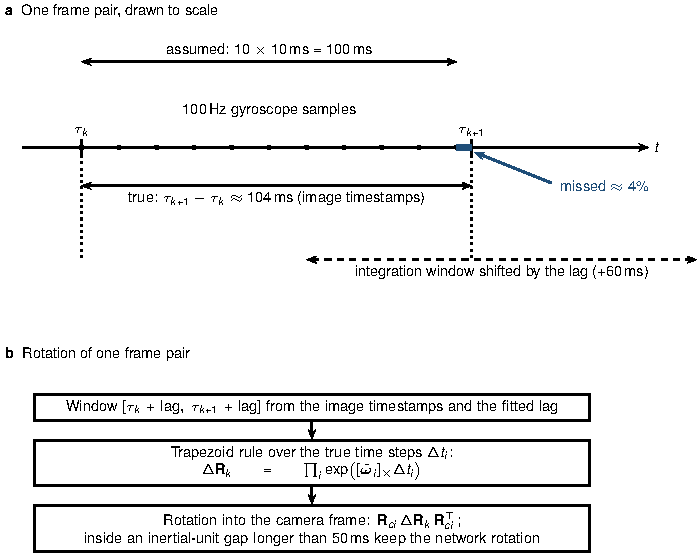
\includegraphics[width=0.9\textwidth]{figures/timing.pdf}
\caption{\tbf{Gyroscope rotation over the true image interval.} \tbf{a}, The released inertial windows hold 11 samples per image pair, read as ten steps of 10 ms, but the image interval is about 104 ms, so every frame pair loses about 4\% of its rotation (blue). \tbf{b}, Processing of one frame pair. The lag and the IMU-to-camera rotation $\mathbf{R}_{ci}$ are fitted on training drives only: the lag on a grid from $-80$ to $+80$ ms (steps of 10 ms, then 2.5 ms) minimising the median residual after a rigid (Kabsch) alignment.}\label{fig:timing}
\end{figure}

\subsubsection{EuRoC: direction}

On EuRoC, ground-truth rotation gives no gain, while ground-truth translation lowers the ATE below the zero-motion floor on three of four sequences. The learned direction error grows with the distance from the training rooms: for PI-VIFT, our variant of VIFT with additional preintegration inputs (Methods), it is 53$^\circ$ on MH\_05 (four training sequences in the same room), 66$^\circ$ on V2\_02 (one) and 70--90$^\circ$ on V1 (none), approaching a random direction. Neither an up-to-scale direction loss\cite{Wang2020} nor unfreezing the encoder made it transfer (one seed each; ATE 6.60 and 3.60 m). On TUM-VI, where we did not run the swap, the network direction is 40--87$^\circ$ off and its length 14--83\% too long.

\subsection{An observability gate chooses between measurement and network}\label{sec:gate-design}

The gate (Fig.~\ref{fig:pipeline}; details in Methods) decides, for each frame pair and component, whether to use a sensor measurement or the frozen network. Rotation always comes from the gyroscope integrated over the true image interval. The direction comes from two-view geometry, with the gyroscope rotation known, where the parallax is large enough, fused with the network's direction when the two agree within their combined uncertainty, and otherwise taken from geometry where they clearly disagree. The step length comes from a linear alignment of accelerometer data over a window of frame pairs, but only when that window is observable (well conditioned, with the estimated gravity close to 9.81 m s$^{-2}$); elsewhere the network length is kept. The gate uses only signals computable from the sensors: parallax, the uncertainty of the geometric solution, the conditioning of the alignment and the gravity norm. The final form is called version 3 (v3). A later post-hoc version, v4, additionally estimates the network's trustworthiness online.

\begin{figure}[t]
\centering
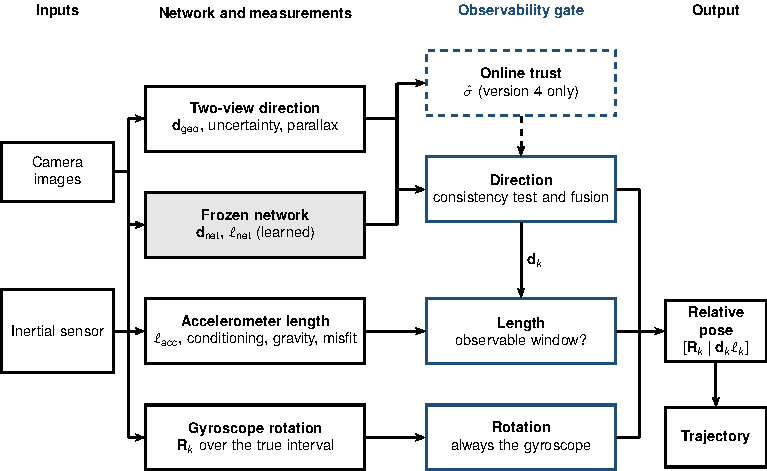
\includegraphics[width=\textwidth]{figures/pipeline.pdf}
\caption{\tbf{Architecture.} The camera and the inertial sensor feed a frozen learned network (shaded; only its direction of translation $\mathbf{d}_\mathrm{net}$ and step length $\ell_\mathrm{net}$ are used) and three measurements that involve no learning. Two-view direction uses the gyroscope rotation, and accelerometer length uses the gyroscope attitudes; each measurement comes with a quality signal. The observability gate (blue outline) combines them for every frame pair and component. The dashed online-trust block belongs to the post-hoc version 4 only and estimates how far the network can be trusted from its agreement with confident geometry. Details of the network and of the gate decisions are in Supplementary Figs.~S1--S3.}\label{fig:pipeline}
\end{figure}

\textbf{Evaluation protocol.} The released code of the base network trains on drive 08 although its paper excludes it, and selects checkpoints on the test drives. Our headline (\emph{clean}) protocol uses the split of the paper's text and selects the checkpoint on held-out drive 08; the split of the released code, with checkpoints selected on the test drives as in the released code, is reported as secondary. The gate constants were fixed on training or held-out data, and the success criterion was registered before a single test run: to match or beat the better hand-designed pipeline within 0.05 $t_\mathrm{rel}$ (KITTI) or 0.1 m (EuRoC, TUM-VI), where a hand-designed pipeline is one in which we fixed by hand which components are measured and which are learned. One deviation occurred: the registered text required both length checks (condition number and gravity norm) on every dataset, while the code that produced all results applies one per dataset. The repeat with both checks leaves the results unchanged (Methods).

\subsection{KITTI}

Table~\ref{tab:kitti} gives the main result. The gyroscope removes most of the error (3.04 to 2.10\% on the clean split, $r_\mathrm{rel}$ 1.04 to 0.18; Fig.~\ref{fig:heading}), the accelerometer length most of the rest (1.62\%), and the gate, which measures the length and fuses the direction, reaches 1.56\% without test-set selection, against the 1.96\% reported for VIFT. The value $r_\mathrm{rel}=0.18$ is measured against OXTS, which shares its inertial unit with the gyroscope; against the lidar-SLAM poses of SuMa\cite{Behley2018}, which do not use the IMU, it is 0.32, close to the 0.25 disagreement between the two references. Against SuMa the numbers rise by about 0.1 point (1.65\%), and a calibration that never touches OXTS ground truth (factory extrinsic, lag fitted against SuMa) gives 1.69\% for the hand-designed pipeline, so the gain is not an artefact of the inertial unit and the ground truth sharing a source. On the split of the released code the gate reaches 1.21\%. A variant without the network (gyroscope, fixed forward direction, accelerometer length, median length where unobservable) scores only 10.9\%: on a car the length is unobservable at stops and at constant speed, and there the network is needed. One caveat: on held-out drive 08 itself, the gyroscope with network translation (0.86\%) beats both the accelerometer length (1.22\%) and the gate (1.20\%), most likely because the checkpoints were selected on that drive.

\begin{table}[t]
\caption{KITTI drives 05, 07 and 10: $t_\mathrm{rel}$ (\%) (mean $\pm$ standard deviation over 3 training seeds) / $r_\mathrm{rel}$ ($^\circ$ per 100 m). Clean: split of the paper's text, checkpoint selected on held-out drive 08. With 08: checkpoint selected on the test drives, as in the released code. SuMa: lidar-SLAM reference independent of the IMU; against SuMa, $r_\mathrm{rel}$ is 0.32 for every row with gyroscope rotation. Gate v3 and v4 give identical results here.}\label{tab:kitti}
\small
\setlength{\tabcolsep}{3pt}
\begin{tabular}{@{}lccc@{}}
\toprule
 & Clean, OXTS & Clean, SuMa & With 08, OXTS \\
\midrule
Network & 3.04$\pm$0.86 / 1.04 & 3.08 & 2.15$\pm$0.17 / 0.83 \\
+ gyroscope rotation & 2.10$\pm$0.04 / 0.18 & 2.20 & 1.61$\pm$0.07 / 0.18 \\
+ accelerometer length & 1.62$\pm$0.03 / 0.18 & 1.71 & 1.27$\pm$0.07 / 0.18 \\
\tbf{Gate (v3 = v4)} & \tbf{1.56$\pm$0.02} / 0.18 & \tbf{1.65} & \tbf{1.21$\pm$0.06} / 0.18 \\
\bottomrule
\end{tabular}
\end{table}

\begin{figure}[t]
\centering
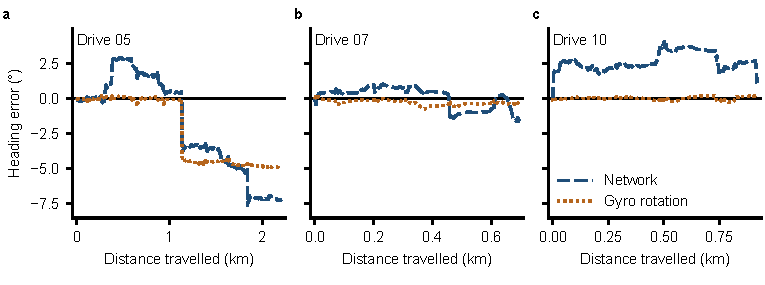
\includegraphics[width=\textwidth]{figures/kitti_heading_error.pdf}
\caption{\tbf{Heading error against distance on KITTI.} Drives 05 (\tbf{a}), 07 (\tbf{b}) and 10 (\tbf{c}). The network heading wanders by 2--7$^\circ$; the gyroscope integrated over the true image intervals stays within about $\pm0.5^\circ$. The step on drive 05 near 1.13 km lies in a 1.62 s outage of the inertial navigation unit and appears in both curves, so it most likely comes from the ground truth.}\label{fig:heading}
\end{figure}

Comparisons with earlier work are in Supplementary Table~S3. On KITTI the gate lowers $t_\mathrm{rel}$ by 0.13--0.40 points against learned VIO on a comparable or stricter protocol, and $r_\mathrm{rel}$ by 61--74\%; against DAP-Pose with satellite positioning the gain is 0.10 points, without it. The earlier numbers come from different protocols and were not rerun, so the comparison is indicative only.

\subsection{Cross-model check}

To test whether the diagnosis and the gate transfer to models we did not train, we ran the same chain, with the gate frozen and run once, on VS-VIO\cite{Yang2022} with its authors' weights (learned visual policy). The error falls from 2.35\% (network) to 1.81\% (gyroscope, $r_\mathrm{rel}$ 0.88 to 0.17), 1.38\% (accelerometer length) and 1.27\% (gate; 1.30\% against SuMa); with full vision it falls from 3.88 to 1.59\%. Table~\ref{tab:gate} adds the same chain run once on the released weights of UL-VIO\cite{Park2024ULVIO} and of the two NASVIO variants\cite{Chen2023NASVIO}: the gate lowers their error by 45--51\% ($t_\mathrm{rel}$ 3.52 to 1.74, 2.58 to 1.42 and 2.50 to 1.38\%). All were trained with drive 08 in their split, so these are with-08 numbers.

\subsection{EuRoC}

On EuRoC (Table~\ref{tab:euroc}) the learned models sit above the zero-motion floor, while measuring every component without a network gives 1.02 m. The gyroscope rotation is accurate to 0.008--0.021$^\circ$ per frame pair, the two-view direction to 1.1--2.0$^\circ$, and the accelerometer length to within 0.7--5\% (all except on V1\_01, discussed below). Geometry is available on 85--96\% of the frame pairs, and the gate, with the same configuration as on KITTI, reaches 0.94--0.99 m. Classical VIO remains far ahead (ORB-SLAM3\cite{Campos2021}, run by us under the same protocol: 0.042 m), so this result is a diagnosis of where learned VIO fails, not a state of the art on EuRoC.

\begin{table}[t]
\caption{EuRoC: ATE (m) on the 10 Hz chain of frame pairs, after rigid alignment (SE(3)); VINS-Mono is as reported in the literature, after similarity alignment (Sim(3), which also fits the scale). The network-free pipeline and the gate use the same sensors as the networks (left camera and IMU). Learned networks: a base-style network and PI-VIFT. Gate v3 is shown for two networks (two values).}\label{tab:euroc}
\small
\setlength{\tabcolsep}{3pt}
\begin{tabular}{@{}lccccc@{}}
\toprule
 & MH\_05 & V2\_02 & V1\_01 & V1\_02 & Mean \\
\midrule
Zero-motion floor & 6.84 & 2.12 & 1.85 & 1.77 & 3.15 \\
Learned networks & -- & -- & -- & -- & 4.02--4.98 \\
Network-free (measured only) & 1.00 & 0.24 & 2.47 & 0.35 & 1.02 \\
\tbf{Gate v3} & -- & -- & -- & -- & \tbf{0.94 / 0.99} \\
ORB-SLAM3, our run, no loop closure & 0.060 & 0.047 & 0.037 & 0.024 & 0.042 \\
VINS-Mono\cite{Delmerico2018}, literature & 0.35 & 0.08 & 0.07 & 0.10 & 0.15 \\
\bottomrule
\end{tabular}
\end{table}

Sequence V1\_01 is above the floor for every learned and per-frame-pair method. A check of every frame pair shows that V1\_01 never rests, so our static-start gyroscope bias fell back to zero while the true bias is about 0.076 rad s$^{-1}$, a 0.46$^\circ$ rotation error per frame pair that biases every geometric direction. Estimating the bias from visual rotations instead (an offline estimate over the whole sequence, agreeing with the static bias within 0.003 rad s$^{-1}$ on the other sequences) brings V1\_01 to 0.92 m without a network and 0.60 m with the gate. Because this was found on a test sequence, we report it as a diagnostic and keep the original numbers.

\subsection{TUM-VI and the gate across datasets}\label{sec:tumvi}

TUM-VI tests transfer to a handheld fisheye platform with motion-capture ground truth. Before any network output, each measurement was checked on the test rooms: gyroscope rotation 0.13--0.16$^\circ$ per frame pair, two-view direction 0.88--1.27$^\circ$ (fisheye) and accelerometer length within 0.5\%. The network-free pipeline scores 0.80 and 0.13 m on room5 and room6; on room5 it loses accuracy on steps shorter than 3 cm. ORB-SLAM3 scores 0.028 m.

\begin{table}[t]
\caption{Gate v3 (pre-registered) and v4 (post-hoc, frozen, run once) across datasets. KITTI: $t_\mathrm{rel}$ (\%); EuRoC and TUM-VI: ATE (m). Hand-designed: best pipeline in which we fixed by hand which components are measured and which are learned. Rows marked with a dagger ($\dagger$): released weights of models we did not train, trained with drive 08, so with-08 numbers against OXTS; v3 and v4 were run once, frozen, and v4 was designed without these models. VS-VIO: learned visual policy / full vision. EuRoC, two sequences: five models. TUM-VI: three training seeds (123, 42, 7).}\label{tab:gate}
\footnotesize
\setlength{\tabcolsep}{2.3pt}
\begin{tabular}{@{}lcccc@{}}
\toprule
Dataset & Network & Hand-designed & Gate v3 & Gate v4 \\
\midrule
KITTI clean (OXTS / SuMa) & 3.04 / 3.08 & 1.62 / 1.71 & 1.56 / 1.65 & 1.56 / 1.65 \\
KITTI with 08 & 2.15 & 1.27 & 1.21 & 1.21 \\
VS-VIO\cite{Yang2022}, policy / full vision & 2.35 / 3.88 & 1.38 / 1.69 & 1.27 / 1.59 & 1.27 / 1.59 \\
UL-VIO\cite{Park2024ULVIO} $\dagger$ & 3.52 & 1.82 & 1.74 & 1.74 \\
NASVIO FLOPs variant\cite{Chen2023NASVIO} $\dagger$ & 2.58 & 1.47 & 1.42 & 1.42 \\
NASVIO latency variant\cite{Chen2023NASVIO} $\dagger$ & 2.50 & 1.43 & 1.38 & 1.38 \\
EuRoC, four sequences (two models) & 5.47 / 6.60 & 1.02 & 0.94 / 0.99 & 0.95 / 0.98 \\
EuRoC, two sequences (five models) & 3.98--5.30 & 0.62 & 0.66--0.90 & \tbf{0.57--0.59} \\
TUM-VI, three seeds & 5.0--8.8 & 0.47 & 0.56 / 0.92 / 0.59 & \tbf{0.47 / 0.47 / 0.47} \\
\bottomrule
\end{tabular}
\end{table}

\textbf{Pre-registered result (v3).} In Table~\ref{tab:gate}, without being told the dataset, the gate meets the criterion on KITTI and on the EuRoC four-sequence means, and, run frozen on VS-VIO, beats the hand-designed chain there. On the two-sequence EuRoC runs, 3 of 5 models miss the 0.1 m tolerance. On TUM-VI it fails: 0.69 m mean over three seeds against a limit of 0.57 m, most of the loss on room5. Before v3, the pre-registered version 1 and a post-hoc version 2 had failed on KITTI, and those test results informed the diagnosis (Supplementary Table~S1); v3 itself was designed only on held-out drive 08.

\textbf{Why it fails, and v4.} The gate assumes that the network's direction error is $\sigma_\mathrm{net}=0.83^\circ$, its value on KITTI. On TUM-VI the network is tens of degrees off, so wherever it happens to agree with geometry the fusion over-weights it, and frame pairs without geometry inherit its direction. Version 4 replaces the fixed value by an online estimate $\hat\sigma$ of the network error (Methods). It was designed only on held-out data: KITTI drive 08 and zero-shot predictions on TUM-VI rooms 1--4. There $\hat\sigma$ recovers the KITTI value without ground truth (0.77--0.80$^\circ$ against 0.83$^\circ$) and flags the TUM-VI network as unreliable (25--74$^\circ$); a pre-declared rule selected the threshold $\tau=10^\circ$. Run once on every test set, v4 equals v3 where the network is good (KITTI and all released models; $\hat\sigma\approx0.65$--$0.9^\circ$ on UL-VIO and NASVIO), fixes the two-sequence EuRoC runs (0.57--0.59 m against 0.62 m hand-designed) and reaches 0.47 m on all TUM-VI seeds. There it equals the network-free pipeline: the gate stops doing harm, but the network adds nothing. Because v4 was motivated by a test failure and the KITTI and EuRoC test sets had been used in earlier gate runs, we label it post-hoc. On EuRoC sequence V2\_03, which was used at no stage, $\hat\sigma$ reads 59--70$^\circ$ against a network error of 61--72$^\circ$; v3 and v4 cut the error from 3.4 m to 2.0 and 2.1 m, so v4 is no better than v3. Any $\tau$ from 3 to 20$^\circ$ gives identical results.

\begin{figure}[t]
\centering
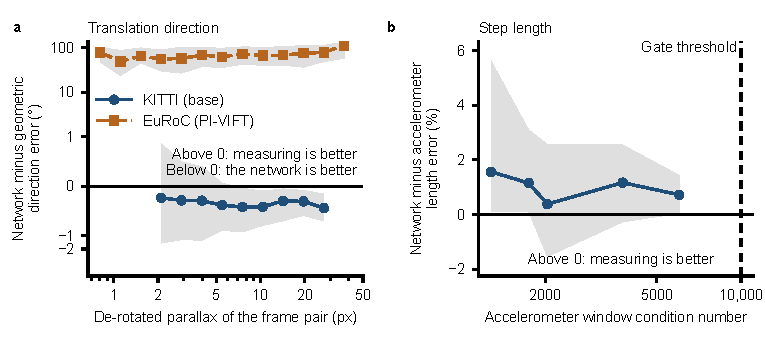
\includegraphics[width=\textwidth]{figures/observability_measure_vs_learn.pdf}
\caption{\tbf{When to measure and when to learn.} \tbf{a}, Network minus geometric direction error against de-rotated parallax (lines: bin medians; bands: interquartile range). On EuRoC, measuring is better by 50--110$^\circ$; on KITTI the network is better by 0.3--0.5$^\circ$. \tbf{b}, KITTI network minus accelerometer length error against the condition number of the window; below the gate threshold the accelerometer is better.}\label{fig:observ}
\end{figure}

\subsection{Design history and constants}

Version 1 (pre-registered) switched to geometry when the angle between network and geometric directions exceeded $3\sqrt{\sigma_\mathrm{geo}^2+\mathrm{FLOOR}^2}$, with a constant FLOOR of 0.685$^\circ$, the median geometric error on KITTI training drives. It met the criterion on EuRoC (1.01 and 0.98 m) but not on KITTI (with 08: 1.96\% and 2.02\% against 1.27\% and 1.32\% for the hand-designed pipeline; clean: 2.31\% and 2.38\% against 1.62\% and 1.71\%). It sent 10--19\% of the frame pairs to geometry, the slow ones (median step 0.28--0.47 m against 0.7--0.86 m overall), where the geometric error is about 2.5$^\circ$ while the predicted uncertainty $\sigma_\mathrm{geo}$ is about 0.13$^\circ$: a floor in degrees is the wrong error model, since the error grows as the parallax shrinks. Version 2 (post-hoc) models the floor in pixels; EuRoC was unchanged (1.00 and 0.96 m) and KITTI still failed (1.99\% and 2.05\%, geometry used on 7\% of the frame pairs). Version 3 adds the inverse-variance fusion and the double length solve, was chosen among several candidates on held-out drive 08, and ran once on the test data (Supplementary Table~S1).

The constants of the gate were fixed before the test results they affect: the factor 3 (a conventional 3-sigma bound), the condition-number bound $10^4$ for 500-frame-pair windows, the gravity tolerance 0.5 m s$^{-2}$ and the 50 ms limit on gaps of the inertial navigation unit. Only the condition-number bound has a sensitivity analysis (Supplementary Table~S2): the test result is identical from $10^4$ to $10^6$, and at $10^3$ almost every window falls back to the network. No sensitivity was run for the factor 3, the gap limit or the lag search range ($-80$ to $+80$ ms, fitted lags $+60$ to $+65$ ms). Without the fallback, IMU-only lengths are fragile on the training drives (2--9\% error on drives 02 and 08). With both length checks everywhere, as registered, the gate results are unchanged on KITTI (released models and three runs of our retrained base network; the clean seeds were not repeated), EuRoC and TUM-VI. The 20-frame-pair bound was chosen on EuRoC training sequences by a prewritten rule and is non-binding; the KITTI bound applied to EuRoC worsens the gate (0.94 to 1.23 m).

\section{Discussion}\label{sec:discussion}

Learned VIO fails in identifiable, dataset-dependent places, and an oracle swap finds them. The useful split between measured and learned components follows observability and differs between datasets (Fig.~\ref{fig:observ}), and the trust placed in the learned part should itself be measured, not assumed. A cheap oracle swap tells which component to fix first; on KITTI it avoids a search for better rotation losses. Measuring what the sensors observe, keeping the network only for the rest, and measuring how far to trust it yields a single configuration that improves the base network to 1.56\% on KITTI without test-set selection, brings EuRoC from 5.5--6.6 m to below 1 m, improves released models from three families we did not train and, once its trust is estimated online (post-hoc), limits the harm on a third dataset.

The work has limitations. (i) On KITTI the IMU and the ground truth share the same OXTS unit; SuMa and a calibration free of OXTS bound this effect (about +0.1 point in $t_\mathrm{rel}$, and $r_\mathrm{rel}$ from 0.18 to 0.32), and TUM-VI motion capture validates the estimators independently. (ii) Version 4 is post-hoc and, on the unseen sequence V2\_03, no better than v3: its gain is shown on TUM-VI only. (iii) The gate cannot beat its measurements: where neither geometry nor the network is reliable (the sub-3 cm steps of TUM-VI room5) nothing helps. (iv) The length check as implemented differs between datasets (condition number on KITTI, gravity on EuRoC and TUM-VI); with both everywhere the results are unchanged, but the bound for 20-frame-pair windows is non-binding. The pixel constants were not rescaled per camera. (v) Estimation from one frame pair to the next, without windowed optimisation, remains about 25 times behind ORB-SLAM3 as run by us and 7 times behind VINS-Mono as reported. (vi) The gyroscope bias needs a static start; an online estimate is future work. (vii) The translation of PI-VIFT contains IMU-preintegrated displacement (Methods), so on EuRoC and TUM-VI the comparison between network length and accelerometer length is not between independent sources; we did not measure how much this matters. (viii) The factor 3, the gap limit and the lag range were fixed without sensitivity analysis.

Natural next steps are networks that predict only the unobservable components together with their uncertainty, and windowed optimisation over the gated estimates.

\section{Methods}\label{sec:methods}

\subsection{Datasets}

KITTI odometry\cite{Geiger2012}: training drives 00, 01, 02, 04, 06 and 09, plus drive 08 in one split; test drives 05, 07 and 10. EuRoC\cite{Burri2016}: training MH\_01--04 and V2\_01, validation V1\_03, test MH\_05, V2\_02, V1\_01 and V1\_02, with the ground-truth quaternion order corrected. TUM-VI\cite{Schubert2018}: training room1--4, test room5--6; 16-bit frames were converted to 8 bits, since a naive conversion saturates every frame. Each frame pair is two consecutive images about 100 ms apart; its relative pose is $[\mathbf{R}_k\,|\,\mathbf{d}_k\ell_k]$ with rotation $\mathbf{R}_k$, unit direction $\mathbf{d}_k$ and length $\ell_k$.

\subsection{Networks and training}

KITTI: the base network, retrained with our recipe (angle-weighted L1 loss), 3 seeds per split, with mirror augmentation on the clean split. EuRoC: a base-style network and PI-VIFT, 3 seeds each; the four-sequence gate runs use PI-VIFT seed 123 and a single-seed PI-VIFT trained with a direction loss. TUM-VI: PI-VIFT fine-tuned from the EuRoC checkpoints, 3 seeds. Cross-model: VS-VIO\cite{Yang2022}, UL-VIO\cite{Park2024ULVIO} and NASVIO\cite{Chen2023NASVIO} with their released weights. No network is retrained for the gate.

\subsection{The learned branch and PI-VIFT}\label{sec:learned}

On KITTI the learned branch is the base network, the released transformer model VIFT\cite{Kurt2024} (Supplementary Fig.~S1): frozen visual and inertial encoders map the stacked frame pair ($256\times512$ pixels) and the 11 interpolated IMU samples to a 768-dimensional latent vector, and a causal transformer over the last 10 latents (4 layers, 6 attention heads) regresses a six-degree-of-freedom relative pose. The gate uses only the translation, split into direction $\dnet$ and length $\ell_\mathrm{net}$; the predicted rotation is discarded in favour of the gyroscope. On EuRoC and TUM-VI we use PI-VIFT (Supplementary Fig.~S2), which keeps the frozen encoders and the causal transformer and changes three things. (i) Two extra tokens enter each frame pair: the preintegration of its IMU window (rotation as a 6-dimensional vector, velocity and position increments and the step time, 13 numbers) and a state token (velocity, gravity and the two biases, 12 numbers), each mapped to 128 dimensions, so the transformer input has 1,024 dimensions. (ii) The output layers produce 18 residual corrections that are added to a kinematic prediction, and a physics step propagates the state from one frame pair to the next and carries it to the next window. (iii) Velocity (weight 0.1) and gravity direction (weight 0.05) are supervised in addition to a multi-horizon pose loss. The physics equations sit in the forward pass, not in the loss, and use only the IMU and the carried state; images enter through the encoder latents. Its translation therefore already contains IMU-integrated displacement, so on EuRoC and TUM-VI the network length is not an independent source relative to the accelerometer.

\subsection{Rotation from the gyroscope}

We integrate the raw gyroscope over the true image interval, $\Delta\mathbf{R}_k=\prod_i \exp([\bar{\boldsymbol{\omega}}_i-\mathbf{b}_g]_\times\,\Delta t_i)$, with the bias $\mathbf{b}_g$ taken from a static start where the sequence has one (EuRoC) and zero otherwise (KITTI, and the TUM-VI rooms, whose bias is below 0.002 rad s$^{-1}$), and rotate it into the camera frame with the calibrated extrinsic rotation (Fig.~\ref{fig:timing}b). Rotation comes from the gyroscope, except inside OXTS outages longer than 50 ms, where the network rotation is kept (effect at most 0.01\%).

\subsection{Direction from two-view geometry}

With $\mathbf{R}_k$ known, each tracked corner pair (bearings $\mathbf{x}_A$, $\mathbf{x}_B$) gives one linear constraint $\mathbf{t}^\top\big((\mathbf{R}_k\mathbf{x}_B)\times\mathbf{x}_A\big)=0$, so two corners fix the direction. We track corners with forward--backward Lucas--Kanade optical flow, undistort them (radial--tangential or equidistant fisheye model, limited to 60$^\circ$ off the optical axis), run two-point random sample consensus (RANSAC) with a 1 pixel epipolar threshold, refit on the inliers by singular value decomposition and fix the sign by requiring the points to lie in front of the camera. The first-order uncertainty $\sigma_\mathrm{geo}$ follows from the singular values; below 2 pixels of de-rotated parallax the direction is re-measured over 200 or 300 ms. A frame pair has no geometric direction, and keeps the network's, when fewer than 15 corners are tracked, the median de-rotated parallax is below 0.5 pixels, or RANSAC keeps fewer than 15 inliers or fewer than half of the matches; geometry is available on 85--96\% of the EuRoC frame pairs and on 88--95\% of those of TUM-VI rooms 1--4.

\subsection{Length from the accelerometer}

Over a window of $W$ consecutive frame pairs we solve a linear alignment\cite{Qin2017} for the initial velocity $\mathbf v_0$, gravity $\mathbf g$, accelerometer bias $\mathbf b_a$ (with a ridge prior) and the $W$ step lengths $\ell_k$, given gyroscope attitudes, preintegrated accelerations and the directions $\mathbf d_k$:
\begin{align}
\mathbf R_k\mathbf R_{bs}\,\mathbf d_k\,\ell_k &= \mathbf v_k\Delta t_k+\tfrac12\mathbf g\,\Delta t_k^2\nonumber\\
&\quad+\mathbf R_k(\boldsymbol\alpha_k-\mathbf J_{\alpha,k}\mathbf b_a)+(\mathbf R_{k+1}-\mathbf R_k)\mathbf p_{bs},\label{eq:align}\\
\mathbf v_k &= \mathbf v_0+\mathbf g\,T_k+\textstyle\sum_{j<k}\mathbf R_j(\boldsymbol\beta_j-\mathbf J_{\beta,j}\mathbf b_a),\nonumber
\end{align}
where $\boldsymbol\alpha_k$ and $\boldsymbol\beta_k$ are the position and velocity increments preintegrated from the raw accelerometer over frame pair $k$, $\mathbf J$ their Jacobians with respect to the bias, $\mathbf R_k$ the gyroscope attitude, $\mathbf R_{bs}$ the camera-to-IMU rotation, $\mathbf p_{bs}$ the camera lever arm and $T_k$ the time since the window start. Each frame pair gives three equations, so $3W$ equations are linear in $9+W$ unknowns; a ridge row (weight 1) pulls $\mathbf b_a$ toward zero, and the \emph{alignment misfit} is the root-mean-square of the residuals, in metres. Windows are disjoint; a KITTI window containing an OXTS gap longer than 50 ms keeps the network length. $W$ is 500 frame pairs on KITTI (about 52 s, chosen on training drives) and 20 on EuRoC and TUM-VI (2 s). A window is used if it is observable: its design matrix has a condition number below a bound ($10^4$ for the 500-frame-pair KITTI windows, $10^7$ for the 20-frame-pair EuRoC and TUM-VI windows) and its gravity estimate lies within 0.5 m s$^{-2}$ of 9.81 m s$^{-2}$; otherwise the network length is kept.

\subsection{The observability gate}

Rotation is the gyroscope's. For the direction, let $\sigma_g^2=\sigma_\mathrm{geo}^2+(A/p)^2$, where $p$ is the de-rotated parallax and $A=6.755^\circ$ pixel a floor fitted on KITTI training drives. If $\angle(\dnet,\dgeo)\le 3\sqrt{\sigma_g^2+\sigma_\mathrm{net}^2}$, the two directions are fused with inverse-variance weights; otherwise $\dgeo$ replaces $\dnet$ when the angle exceeds $3\sigma_g$, and $\dnet$ is kept on the remaining frame pairs (Supplementary Fig.~S3). Each length window is solved with both $\dnet$ and the gated direction, keeping the solution with the smaller alignment misfit, so a few wrong directions cannot corrupt a window. In the pre-registered version (v3), $\sigma_\mathrm{net}=0.83^\circ$, the network's median direction error on held-out KITTI drive 08.

\subsection{Online trust (v4)}

A fixed $\sigma_\mathrm{net}$ assumes that the network is as good everywhere as on KITTI. Version 4 estimates it causally without ground truth: $\hat\sigma(k)$ is the median angle between $\dnet$ and $\dgeo$ over the last 100 \emph{confident} frame pairs (geometry present, parallax $p\ge5$ pixels, $\sigma_g\le1^\circ$), with the $0.83^\circ$ prior until 20 such frame pairs exist. If $\hat\sigma>\tau=10^\circ$, frame pairs without geometry hold the last gated direction and the length windows use only the gated direction. The confidence constants were fixed from first principles and $\tau$ was selected on held-out data (Results).

\subsection{Metrics, references and statistics}

KITTI $t_\mathrm{rel}$ and $r_\mathrm{rel}$ are computed over segments of 100--800 m, against the OXTS ground truth and against SuMa lidar-SLAM poses\cite{Behley2018}, which do not use the IMU. EuRoC and TUM-VI errors are the ATE after rigid (SE(3)) alignment of the 10 Hz chain of frame pairs, reported next to the zero-motion floor. Where a table gives $\pm$, it is the standard deviation over three training seeds; the other entries are single runs or ranges across runs, as stated. We report no hypothesis tests.

\subsection{Runtime}

The measurement side costs 39--41 ms per 100 ms frame pair on one Apple M1 Pro core (512$\times$512 fisheye frames), 2.5 times faster than real time; the network runs unchanged on a graphics processor.

\subsection{Use of large language models}

[TO BE FILLED: state here whether large language models were used in the preparation of the work, as Scientific Reports requires for any use beyond copy-editing.]

\section{Acknowledgements}
[TO BE FILLED: acknowledgements and any funding, with grant numbers; Scientific Reports has no separate Funding section.]

\section{Author contributions}
[TO BE FILLED: roles of N.E.M., M.Z., S.E., S.S., M.H. and R.E.S.]

\section{Data availability}
\raggedright
All experiments use public datasets: KITTI odometry (\url{https://www.cvlibs.net/datasets/kitti}), EuRoC (\url{https://projects.asl.ethz.ch/datasets/doku.php?id=kmavvisualinertialdatasets}) and TUM-VI (\url{https://cvg.cit.tum.de/data/datasets/visual-inertial-dataset}), and the released weights of the cited models. The cached intermediate results and the corrected inertial files are [TO BE FILLED: repository, version and DOI].

\section{Code availability}
\raggedright
[TO BE FILLED: repository, version and DOI for the code of the gate, the oracle-swap scripts and the evaluation scripts.]

\section{Competing interests}
[TO BE FILLED: the authors declare no competing interests, or state them.]

\section{Additional information}
\tbf{Ethics declarations.} Not applicable: the study uses public sensor datasets and involves no human participants, human samples or animals. \tbf{Supplementary information.} Supplementary Figs.~S1--S3 and Supplementary Tables~S1--S3 accompany this paper. \tbf{Correspondence} and requests for materials should be addressed to N.E.M. (nadaelmadah@mans.edu.eg).

{\hbadness=4000 \bibliography{refs}}

\end{document}
